\documentclass[12pt]{article}
\usepackage{fullpage}
\usepackage{subcaption,amsmath,amssymb,mathtools,xparse,graphicx,float,datetime,color,array,graphics,enumerate,tikz,pgfplots,xcolor}
\usepgfplotslibrary{statistics}
\pagestyle{empty}
\newcommand{\D}{\displaystyle}
\setlength{\textheight}{9in} \setlength{\headheight}{.2in}
\setlength{\headsep}{0in} \setlength{\topmargin}{0in}
\begin{document}
\begin{center}
CSCI 6100 Machine Learning From Data\\
Fall 2018\\
\end{center}
\begin{center}
HOMEWORK 12\\
Daniel Southwick\\
661542908\\
southd@rpi.edu
\end{center}
\vspace{.1in}

\noindent {\bf 1. Neural Networks and Back propagation} \\\\
a)\\
\indent We implemented the following neural network of a 2 input, $m$-hidden unit ($m=2$), 1 output sigmoidal neural network. We set all weights to $0.25$:
\begin{figure}[H]
  \centering
  \includegraphics[scale = 0.382]{1_1.png}
  \caption{2-input, 2-hidden layer, 1-output Neural network $($made with draw.io$)$}
  \label{fig:1}
\end{figure}
\indent With $x^{(0)}= \begin{bmatrix} 1\\ 1 \end{bmatrix} $ and weights $= 0.25$. The input to the first layer became: $s^{(1)}= \begin{bmatrix} 0.75\\ 0.75 \end{bmatrix} $. Output of the first layer became:  $x^{(1)}= \begin{bmatrix} 1\\ 0.635\\ 0.635 \end{bmatrix} $. Then from the architecture above, we can get: $s^{(2)}= 0.25*(1+0.635+0.635) = 0.568$. And for the output node, $S(s) = s = 0.568$, $\theta(s) = tanh(s) = 0.514$. In addition, $N = 1$ since there's only one data point, thus $\D E_{in}(w) = \frac{1}{4}(h(x,w)-y)^2$ and:
\begin{align*}\D
\frac{\partial h(x,w)}{\partial w^{(2)}} &= \frac{\partial h}{\partial s^{(2)}} \frac{\partial s^{(2)}}{\partial w^{(2)}} = x^{(1)} \frac{\partial h}{\partial s^{(2)}}  \\
\frac{\partial h(x,w)}{\partial w^{(1)}} &= \frac{\partial h}{\partial s^{(2)}} \frac{\partial s^{(1)}}{\partial w^{(1)}} \frac{\partial x^{(1)}}{\partial s^{(1)}} \frac{\partial s^{(2)}}{\partial x^{(1)}} \\
&= x^{(0)}\frac{\partial h}{\partial s^{(2)}} (1 - tanh^2(s^{(1)}))w^{(2)}
\end{align*}
i)\indent $S(s) = s$:\\
\indent $\D \frac{\partial h}{\partial s^{(2)}} = 1$, so $\D \frac{\partial h(x,w)}{\partial w^{(2)}} =  \begin{bmatrix} 1\\ 0.635 \\ 0.635 \end{bmatrix}$ and $\D \frac{\partial h(x,w)}{\partial w^{(1)}} = 0.25*(1-0.635^2) = 0.149$, and since $w^{(1)}$ is a $3 \times 2$ matrix, we take $\D \frac{\partial h(x,w)}{\partial w^{(1)}} = \begin{bmatrix} 0.149 & 0.149\\ 0.149 & 0.149\\ 0.149 & 0.149 \end{bmatrix} $. Now, we compute the Gradient of $E_{in}(w)$ by:
\begin{align*} \D
G_2 = \frac{1}{2}\frac{\partial h(x,w)}{\partial w^{(2)}}(s^{(2)} - y) &= \begin{bmatrix} -0.216\\ -0.137\\ -0.137 \end{bmatrix} \\
G_1 = \frac{1}{2}\frac{\partial h(x,w)}{\partial w^{(1)}}(s^{(2)} - y) &= \begin{bmatrix} -0.032 & -0.032\\ -0.032 & -0.032\\ -0.032 & -0.032 \end{bmatrix} 
\end{align*}
ii)\indent $\theta(s) = tanh(s)$:\\
\indent Follow the same procedure, except $\D \frac{\partial h}{\partial s^{(2)}} = 1 - tanh^2(s) = 0.736$, we can get to: 
\begin{align*} \D
G_2 &= \frac{1}{2}\frac{\partial h(x,w)}{\partial w^{(2)}}(s^{(2)} - y) = \frac{1}{2} \begin{bmatrix} 1\\ 0.635\\ 0.635 \end{bmatrix} 0.736 *(0.513 - 1)^2\\
&= \begin{bmatrix} -0.180\\ -0.114\\ -0.114 \end{bmatrix} \\
G_1 &= \frac{1}{2}\frac{\partial h(x,w)}{\partial w^{(1)}}(s^{(2)} - y) = \frac{1}{2} \begin{bmatrix} 1&1\\ 1&1 \\ 1&1 \end{bmatrix} 0.25*(0.513 - 1)*(1 - 0.513)^2*(1 - 0.635)^2 \\
&=\begin{bmatrix} -0.027 & -0.027\\ -0.027 & -0.027\\ -0.027 & -0.027 \end{bmatrix} 
\end{align*}
b)\\ 
\indent We perturbed each weight in turn by 0.0001 and obtained the following result:\\
i)\indent $S(s) = s$:
\begin{align*} \D
G_2 &=  \begin{bmatrix} -0.216\\ -0.137\\ -0.137 \end{bmatrix}; G_1= \begin{bmatrix} -0.032 & -0.032\\ -0.032 & -0.032\\ -0.032 & -0.032 \end{bmatrix} 
\end{align*}
ii)\indent $\theta(s) = tanh(s)$:
\begin{align*} \D
G_2 &=  \begin{bmatrix} -0.179\\ -0.114\\ -0.114 \end{bmatrix}; G_1= =\begin{bmatrix} -0.025 & -0.025\\ -0.025 & -0.025\\ -0.025 & -0.025 \end{bmatrix} 
\end{align*}
\indent The results are almost all equal to the analysis results in part a), which verified our back propagation gradient calculation.

\newpage
\noindent {\bf 2. Neural Networks for Digits} \\\\
a)\\
\indent We use the Neural Network Model from the previous part, with the new $m=10$, with all active functions being sigmoids. And we put our previous two features from digit 1 and digit 5, Intensity and Asymmetry as our $X1$ and $X2$ input, with $N=300$. We then compute $$\D E_{in}(w) = \frac{1}{300}\sum^{300}_{n=1}(h(x_n,w)-y_n)^2$$ \indent With our max iteration of $2\times 10^{6}$ and $S(x) = x$, the decision boundary at  our max iteration and the iteration errors along the way are shown as follows:
\begin{figure}[H]
\centering
\begin{subfigure}{.5\textwidth}
  \centering
   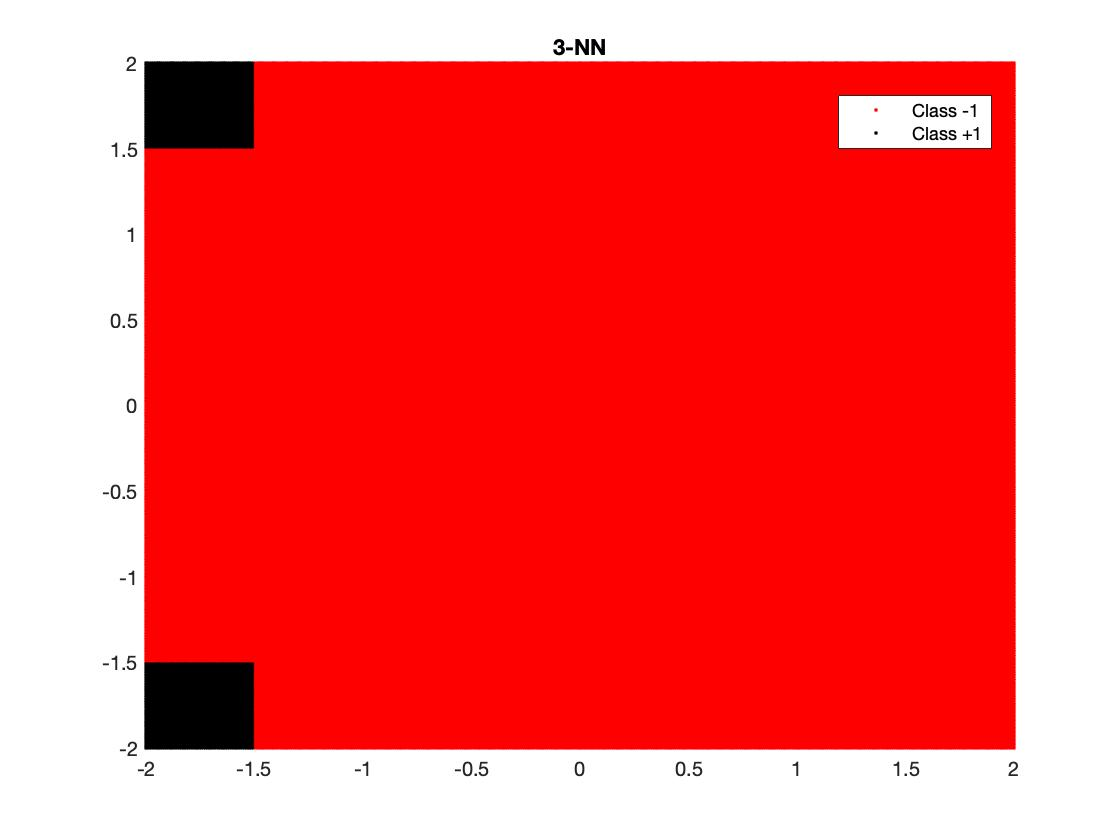
\includegraphics[scale = 0.5]{2.png}
  \caption{Decision Boundary for $S(x) = x$}
  \label{fig:1}
\end{subfigure}%
\begin{subfigure}{.5\textwidth}
  \centering
   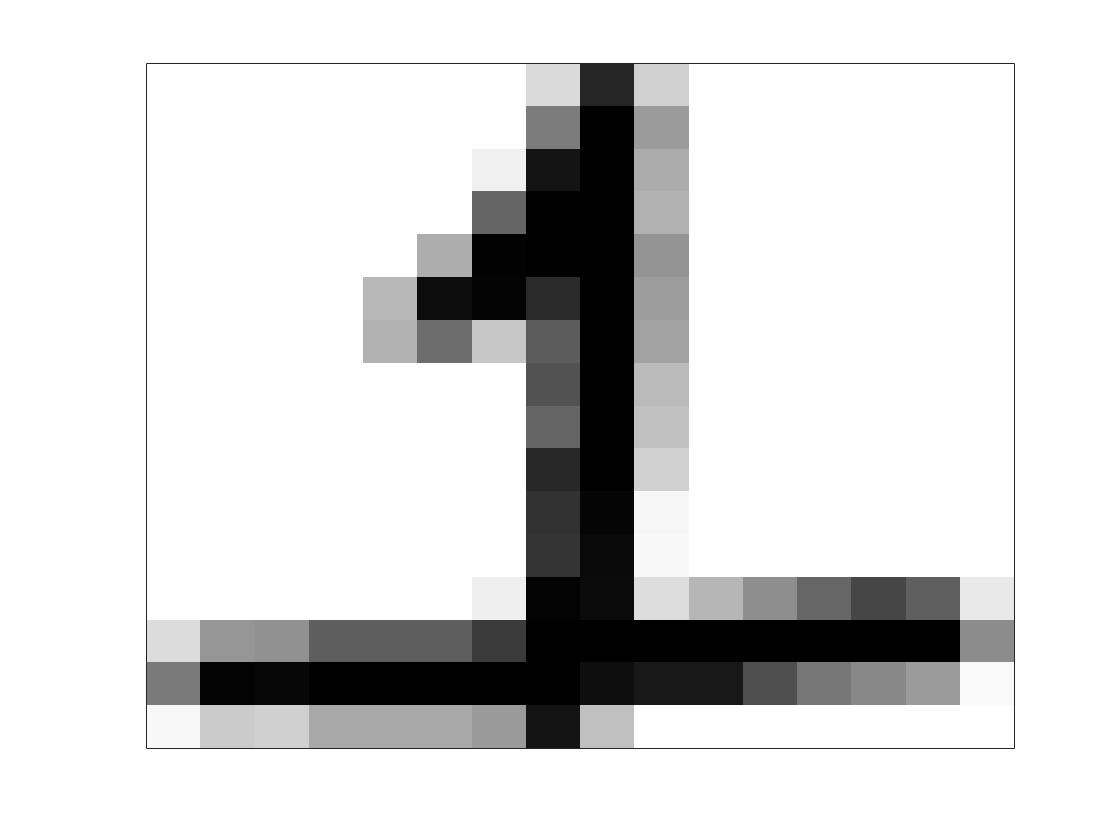
\includegraphics[scale = 0.5]{1.png}
  \caption{$E_{in}$ for $S(x) = x$}
  \label{fig:2}
\end{subfigure}
\caption{$S(x) = x$, Max Iteration $= 2\times 10^6$ }
\label{fig:test}
\end{figure}\indent\\
b)\\
\indent Now, with the weight decay $\D \lambda = \frac{0.01}{N} = \frac{0.01}{300}$, we add the weight decay to previous $E_{in}$, with $N=300$: $$\D E_{in}(w) = \frac{1}{300}\sum^{300}_{n=1}(h(x_n,w)-y_n)^2 + \frac{\lambda}{N}\sum_{l,i,j}(w^l(i,j))^2$$ \indent And follow the same procedure above, With our max iteration of $2\times 10^{6}$ and $S(x) = x$, the decision boundary at  our max iteration and the iteration errors along the way are shown as follows:
\begin{figure}[H]
\centering
\begin{subfigure}{.5\textwidth}
  \centering
   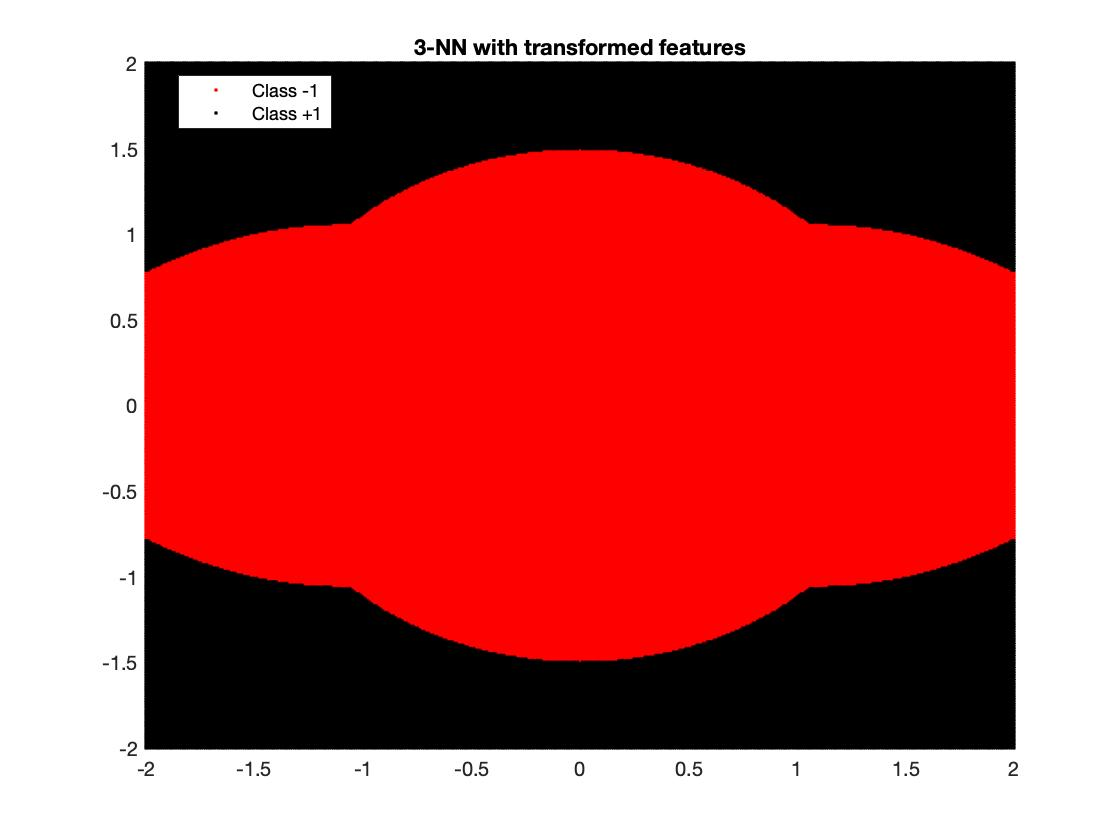
\includegraphics[scale = 0.5]{4.png}
  \caption{Decision Boundary with $\lambda$}
  \label{fig:1}
\end{subfigure}%
\begin{subfigure}{.5\textwidth}
  \centering
   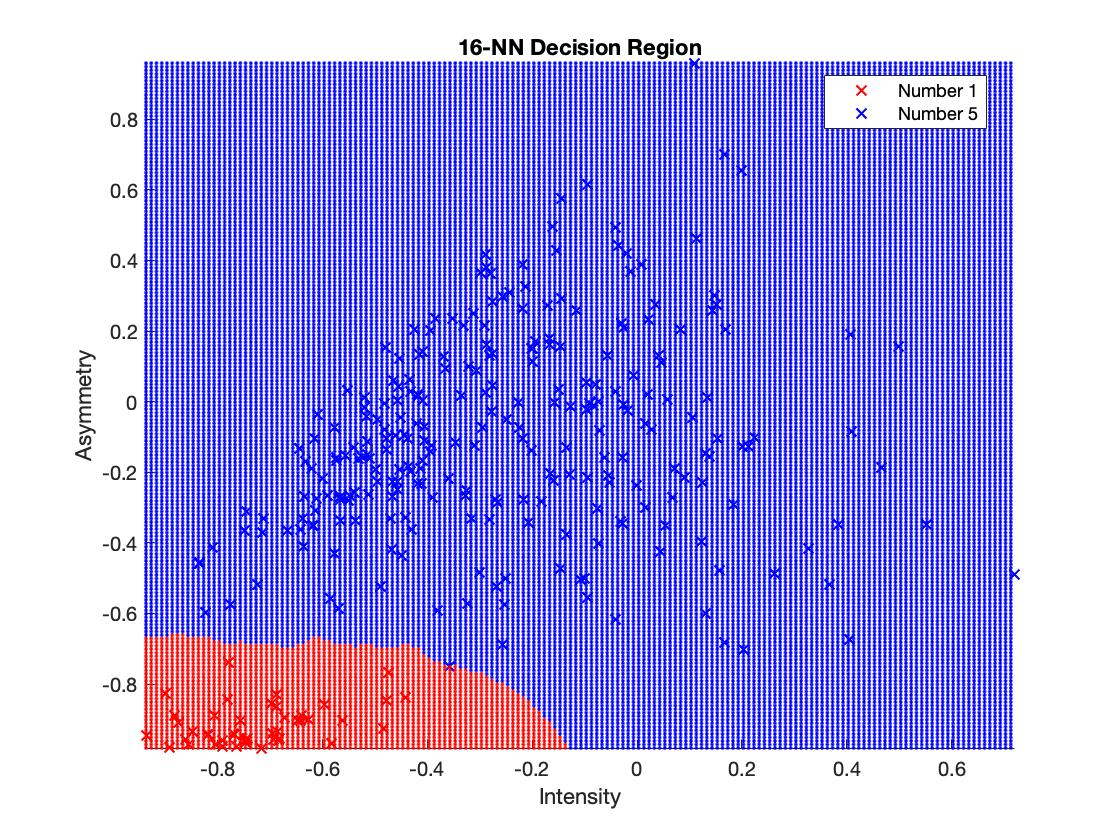
\includegraphics[scale = 0.5]{3.png}
  \caption{$E_{in}$ for $S(x) = x$ with $\lambda$}
  \label{fig:2}
\end{subfigure}
\caption{$S(x) = x$, Max Iteration $= 2\times 10^6$ with weight decay $\lambda = \frac{0.01}{300}$}
\label{fig:test}
\end{figure}\indent\\
c)\\
\indent We then separate the 300 data points into a validation set of size 50 and training set of size 250, so $\D E_{val}(w) = \frac{1}{50}\sum_{n=1}^{50}(\hat{y_n} \neq y_n)$, we count the number of misclassified data within the 50 validation dataset. The minimum $E_{val}(w)$ occurs at iteration $923$ before it goes up again (shown in red curve $Figure$ $4(b)$), in which stopped the iteration, the resulting boundary and the Validation error are shown as follows:
\begin{figure}[H]
\centering
\begin{subfigure}{.5\textwidth}
  \centering
   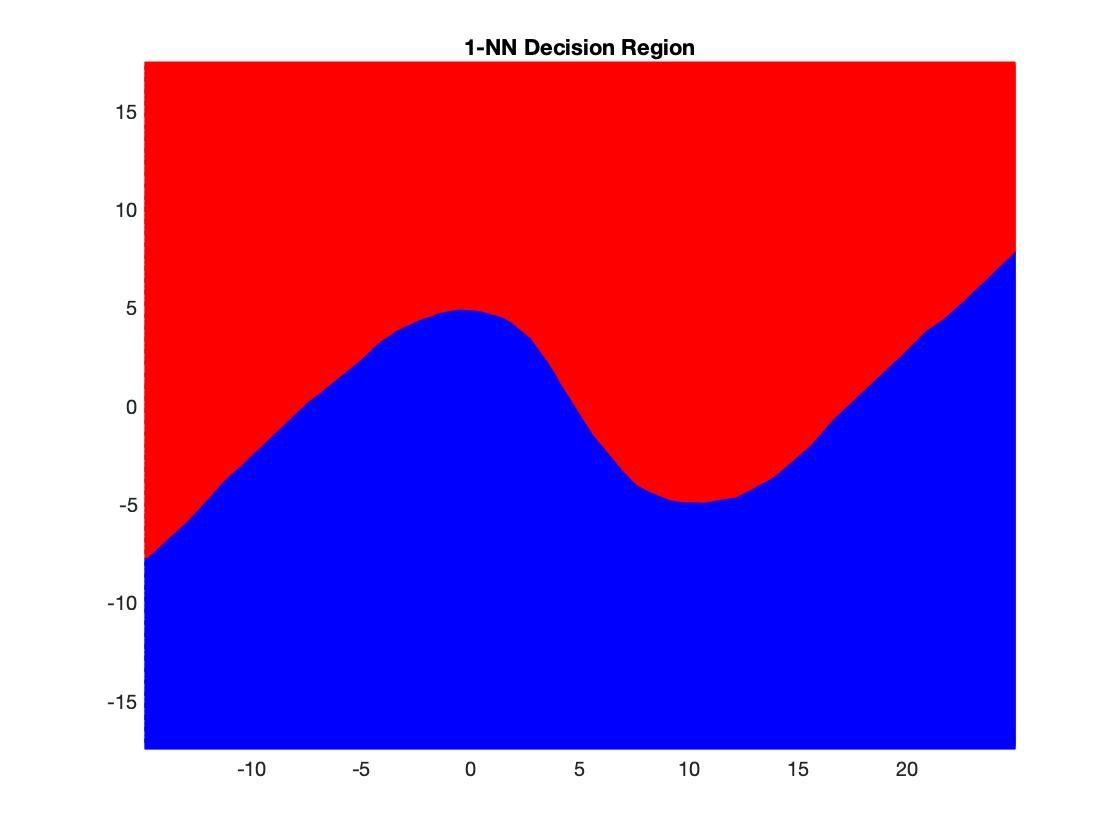
\includegraphics[scale = 0.45]{6.png}
  \caption{Decision Boundary with 923 iterations}
  \label{fig:1}
\end{subfigure}%
\begin{subfigure}{.5\textwidth}
  \centering
   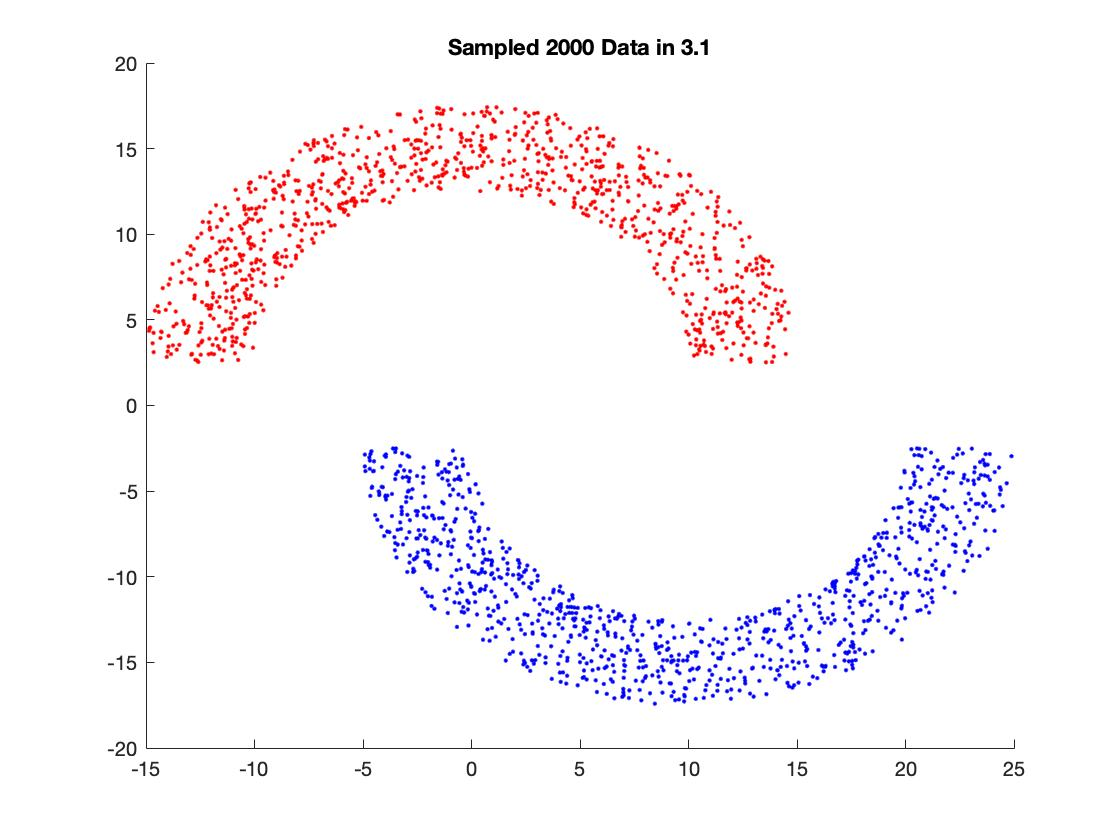
\includegraphics[scale = 0.42]{5.png}
  \caption{$E_{val}$ vs. iterations}
  \label{fig:2}
\end{subfigure}
\caption{$S(x) = x$, Stopping Iteration at iteration $923$}
\label{fig:test}
\end{figure}\indent\\

\noindent {\bf 3. Support Vector Machines} \\\\
a)\\
\indent Since we only have two data points, $x_1 = (1,0), y_1 = +1$ and $x_2 = (-1,0), y_2 = -1$, the hyperplane that separates these two points with the largest wideness of cushion would be a line that's perpendicular to the mid point of $x_1$ and $x_2$, which is $(0,0)$. So the hyperplane is $x_1 = 0$, in other words, the $x_2$-axis.\\\\
b)\\
\indent Now, we consider the transform $\D z = \begin{bmatrix} z_1\\z_2 \end{bmatrix} =  \begin{bmatrix}  x_1^3 - x_2\\x_2x_2 \end{bmatrix}$, so $\D z_1 = \begin{bmatrix}  1 - 0\\1*0 \end{bmatrix} = \begin{bmatrix}  1\\0 \end{bmatrix}$ and $\D z_2 = \begin{bmatrix}  -1 - 0\\(-1)*0 \end{bmatrix} = \begin{bmatrix}  -1\\0 \end{bmatrix}$, here, similar to part a), the hyperplane is $z_1 = 0$ in the $z$ space, so in $x$ space, the boundary is $x_1^3 - x_2 = 0$, note that the boundary is no longer a line like the previous part.\\\\
c)\\
\indent The decision boundaries are shown as follows in the $x$ space and for both $x$ space and the $z$ space:
\begin{figure}[H]
  \centering
  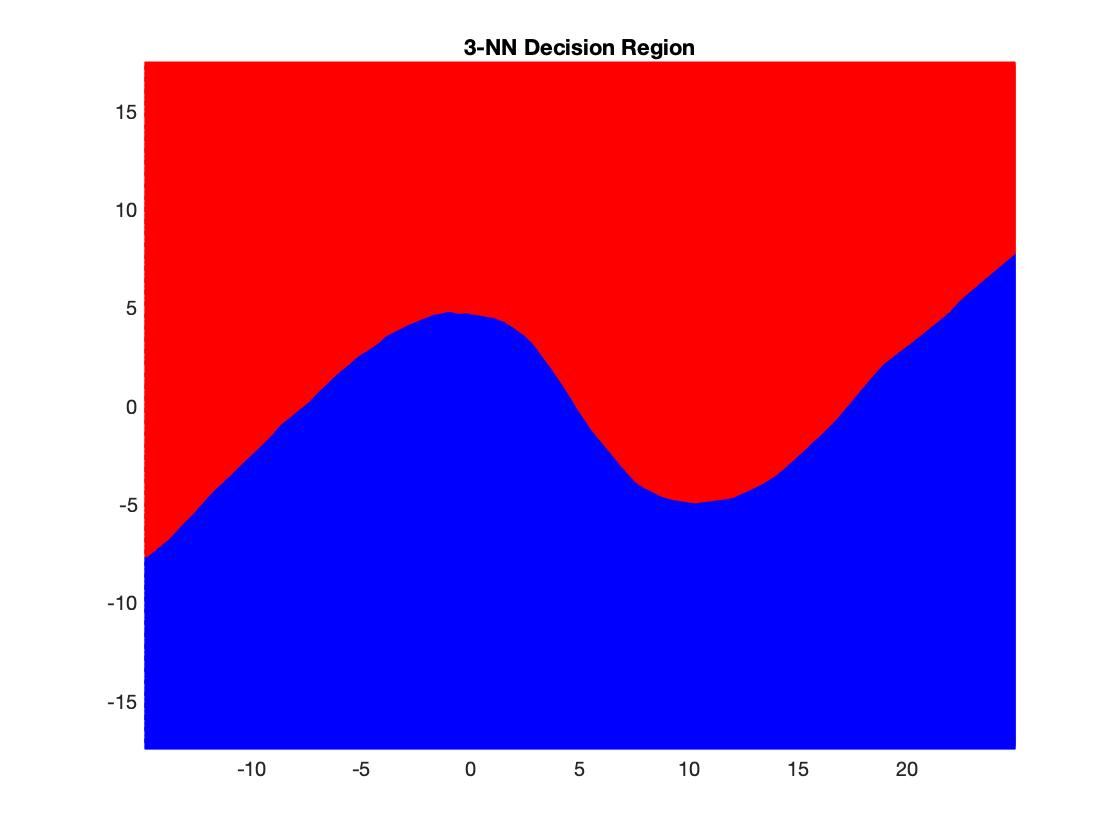
\includegraphics[scale = 0.26]{7.png}
  \caption{SVM Decision boundaries for two points }
  \label{fig:1}
\end{figure}\indent\\
d)\\
\indent The kernel function, $K(x,y) = z(x)\cdot z(y)$'s expression: $$K(x,y) = z(x)\cdot  z(y) =  \begin{bmatrix} x_1^3-x_2\\x_1 x_2 \end{bmatrix} \cdot  \begin{bmatrix} y_1^3-y_2\\y_1y_2 \end{bmatrix} = (x_1^3 - x_2)(y_1^3-y_2)+x_1x_2y_1y_2$$
e)\\
\indent From the previous problem, we have $\D z_1 = \begin{bmatrix} 1\\0 \end{bmatrix}$ and $\D z_2 = \begin{bmatrix} -1\\0 \end{bmatrix}$ and target $y_1 = +1$ and $y_2 = -1$. We ca n set up the decision boundary as follows: $$\D g(x) = sign(\sum_{m,n=1}^{2} y_m\cdot \alpha_n) \cdot K(x,y) +b$$ \indent The optimal solution in this case would be $(\alpha_1, \alpha_2 )= (1/2, 1/2)$, Thus the decision boundaries of the cushion is still $z_1 = 1$ and $z_2 = -1$, and the separating hyperplane is $x_1^3 - x_2 =0$.

\newpage
\noindent {\bf 4. SVM with digits data} \\\\
a)\\
\indent Just like problem 2, we use the same 300 training samples, this time on the non-separable SVM with the 8th order polynomial kernel, $K(x,x^{'}) = (1+x^Tx^{'})^8$. There is an upper bound $C$, the regularizer for each variable $\alpha_i$. The problem now became solving quadratic problem to determine the variables $\alpha_i$. We first tried a relative small $C = 0.001$, and received a large $E_{in} = 0.163$:
\begin{figure}[H]
  \centering
  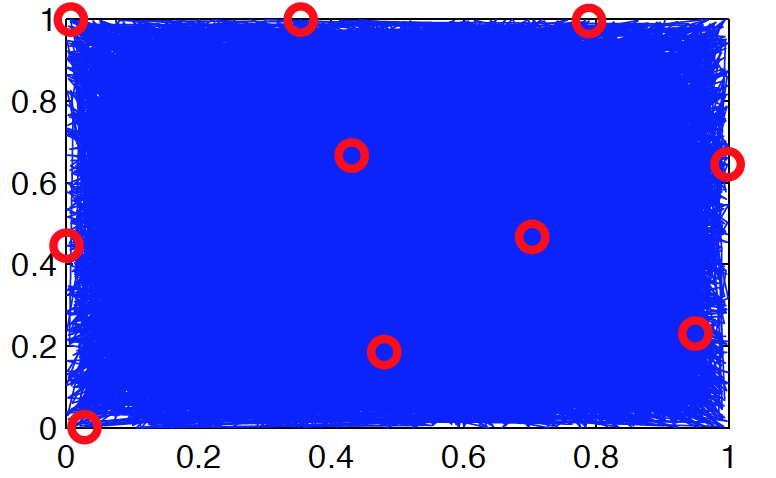
\includegraphics[scale = 0.53]{8.png}
  \caption{SVM Decision boundaries for $C = 0.001$}
  \label{fig:1}
\end{figure}\indent\\
\indent Then we bumped up the $C$ to $10$, and received a pretty small $E_{in} = 0.029$
\begin{figure}[H]
  \centering
  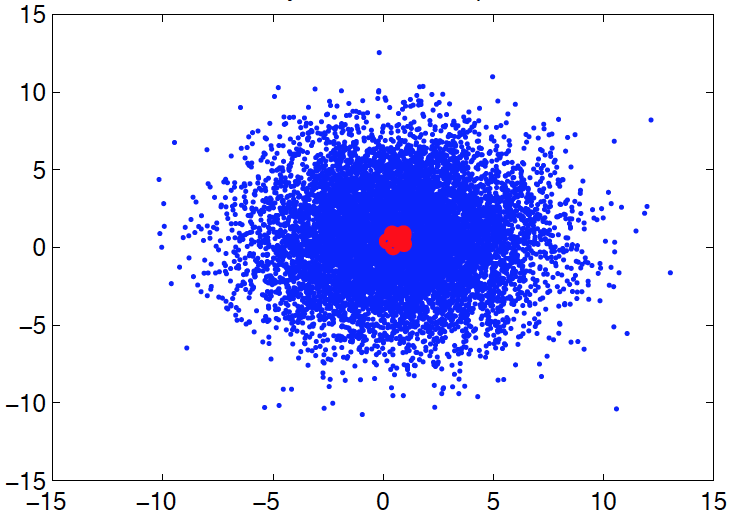
\includegraphics[scale = 0.53]{10.png}
  \caption{SVM Decision boundaries for $C = 10$}
  \label{fig:1}
\end{figure}\indent\\
b)\\
\indent With a higher $C$, we can expect the boundary to be more complex, thus it should fit better to the dataset. Theoretically, a larger $C$ gives a larger penalty to the misclassified samples so there will be more correctly classified samples. The accuracy can also be shown by the significant drop in $E_{in}$. However, I would suspect that once $C$ is large enough, $E_{in}$ would no longer decrease as the algorithm saturates.\\
c)\\
\indent Using the same validation method as our Neural Network, we take 50 points of data out of our 300 training set and make it the cross validations set. $\D E_{cv}(w) = \frac{1}{50}\sum_{n=1}^{50}(\hat{y_n} \neq y_n)$, we count the number of misclassified data within the 50 cross validation dataset and find the percentage. After iterating $C$ over the range of $\left[ 0.001,10 \right]$, we found that the algorithm first reached the minimum $E_{cv} = 0.035$ when $C = 0.1$. We then plotted the boundary:
\begin{figure}[H]
  \centering
  \includegraphics[scale = 0.55]{13.png}
  \caption{SVM Decision boundaries for $C = 0.1$}
  \label{fig:1}
\end{figure}\indent\\

\noindent {\bf 5. Compare Methods: Linear, $k-$NN, RBF-network, Neural network, SVM} \\\\
\indent We have computed the Linear model with 8th order polynomial transform and regularization in HW9, and we recall that the test error is $0.9\%$.  And computed the 16-NN has a test error of $1.57\%$ and RBF has a test error of $1.85\%$ in HW11. Neural network with 923 early stopping has a test error of $1.47\%$ and SVM has a test error of $1.09\%$
Each of these models has its own pros and cons. The linear model with 8th order polynomial transform has the lowest test error rate, the SVM and RBF are similar algorithm and we've compared those in HW11. No matter which method we use, cross validation is necessary to achieve the optimal performance. Linear model and SVM aims to find the separating hyper plane. k-NN and RBF grows the boundary, k-NN grows the boundary from individual data points while RBF uses all data points. Neural network made the combination of different activate function possible.
\end{document}

